\documentclass{bioinfo}
\copyrightyear{2011}
\pubyear{2011}

\begin{document}
\firstpage{1}

\title[a5]{A User-friendly Pipeline for De Novo Genome Assembly}
\author[Tritt \textit{et~al}]{Andrew Tritt\,$^{1}$ Jonathan A. Eisen\,$^{1,2,3}$ Marc T. Facciotti\,$^{1,4}$ and Aaron E. Darling,$^{1}$\footnote{to whom correspondence should be addressed}}
\address{$^{1}$Genome Center, $^{2}$ Dept. of Evolution and Ecology, $^{3}$ Medical Microbiology and Immunology, 
$^{4}$ Biomedical Engineering, University of California-Davis, Davis, CA 95616.}

\history{Received on XXXXX; revised on XXXXX; accepted on XXXXX}

\editor{Associate Editor: XXXXXXX}

\maketitle

\begin{abstract}

\section{Summary:}
Improvements in high throughput DNA sequencing technologies have lead to the development of
many methods for analyzing and processing next-gen data. 
\section{Availability:}
GPL source code and a usage tutorial is at \href{http://ngopt.googlecode.com}{http://ngopt.googlecode.com}

\section{Contact:} \href{rabid apes}{}
\end{abstract}

\section{Introduction}
%De novo genome assembly involves piecing together long sequences from many short sequences.
%These short sequences are often highly erroneous, and target long sequences often contain repetitive 
%elements. 
Advances in high throughput DNA sequencing have lead to an increased demand for de novo 
genome assembly. Numerous pieces of software have been developed for solving this task; 
however, despite many efforts, the task still remains non-trivial. There are many possible
steps that can be taken throughout the process of assembling a genome. At each of these steps,
there exists a plethora of software. However, because of the complexity of the available algorithms,
running such software can be laboreous, as obtaining the optimal result requires manual tuning of parameters.
In addition to being time consuming, parameter tuning requires the user to understand the details
of the algorithms being used. 
%Despite many efforts to solve the problem of genome assembly, the task still remains non-trivial. 

We introduce a new de novo genome assembly pipeline that requires no knowledge
of the underlying algorithms to use. Using previously 
published assembly software and short read tools, our pipeline, A5, carries out
many common steps taken in the genome assembly process. A5 starts with error correction
and removal of contaminant reads, assembly of reads into contigs, and scaffolding
of contigs with paired reads. In addition to these steps, our pipeline performs additional
error checking after scaffolding, to identify and remove any potential misassemblies. 
Our pipeline behaves comparably to many existing assemblers. Although A5 offers no improvement
in assembly quality, time spent running A5 to get optimal results is minimal. 

%De novo genome assembly involves many steps. A lot of software, each of which requires 
%much manual tuning. Rapid growth of high throughput DNA sequence techonologies has made sequence 
%data readily available. Analyzing this data is difficult, in part because 
%assembly algorithms have many parameters that are not easily optimized. 

\begin{methods}
\section{Methods}
The genome assembly problem can be broken down into two main steps: 1) building
contigs and 2) scaffolding contigs. 

We separate building contigs into two steps. The first step in building contigs
is read error correction. For this step we use error correction tools from the
SGA software package to correct reads for sequencing errors. Error corrected reads
are then assembled into contigs using the assembler IDBA. (Do we discuss why we use IDBA?)  

After contigs are built, paired/mated libraries can be used to scaffold contigs 
together. For this stage, our pipeline uses the scaffolder SSPACE. A key 
parameter for scaffolding is the insert size of libraries. Using the read
mapping software package BWA, insert size estimations have been automated. 

After contigs have been scaffolded, reads are mapped back to scaffolds. The locations
of mapped reads and pairing information is used with FISH to identifiy putatively erroneous 
contigs. 



\end{methods}

\subsection{Automated misassembly quality control}

After assembling genomes, an important step is quality control and validation
of "assembly connections". The final step in our pipeline is automated 
misassembly detection. For this step, we use FISH to identify erroneously
connected points in the genome. The FISH algorithm was orignally developed
to identify collinear segments of homology between two genomes. Here, we use
FISH to identify collinear segments of paired read connections between two contigs
or within a single contig. First, reads are mapped onto scaffolds using BWA and 
connected segments are identified using 
FISH. Scaffolds are then broken at the boundaries of these segments and the 
resulting contigs/scaffolds are rescaffolded using SSPACE as described above.


\subsection{Automated parameter selection}

Does this work on non-haloarchaea?


\begin{table}[!t]
\processtable{ Metrics on assemblies of Haloferax volcanii from four pipelines.
\label{Tab:01}}
{\begin{tabular}{l|cccc}\toprule
Metric & volcS & volcV & volcA5 & volcA5-noQC\\\midrule
Scaffold count & 1000 & 10000 & 50  & 6 \\
Miscalled bases & 1000 & 2e6 & 100 & 100 \\
Uncalled bases & 15000 & 60000 & 10000 & 7500 \\
Extra bases & 5.0\% & 2.5\% & 8.0\% & 4.0\% \\
Missing bases & 7.5\% & 13.0\% & 7.5\% & 7.0\% \\
Extra segments & 500 & 262 & 45 & 1 \\
Missing segments & 117 & 1144 & 192 & abc \\
DCJ Distance & 1100 & 10250 & 56 & 8 \\
Intact CDS & 93.2\% & 89.4\% & 97.0\% & 97.3\% \\
\botrule \\
\end{tabular}}{}
\end{table}



\section{Discussion}


\begin{figure}[t]
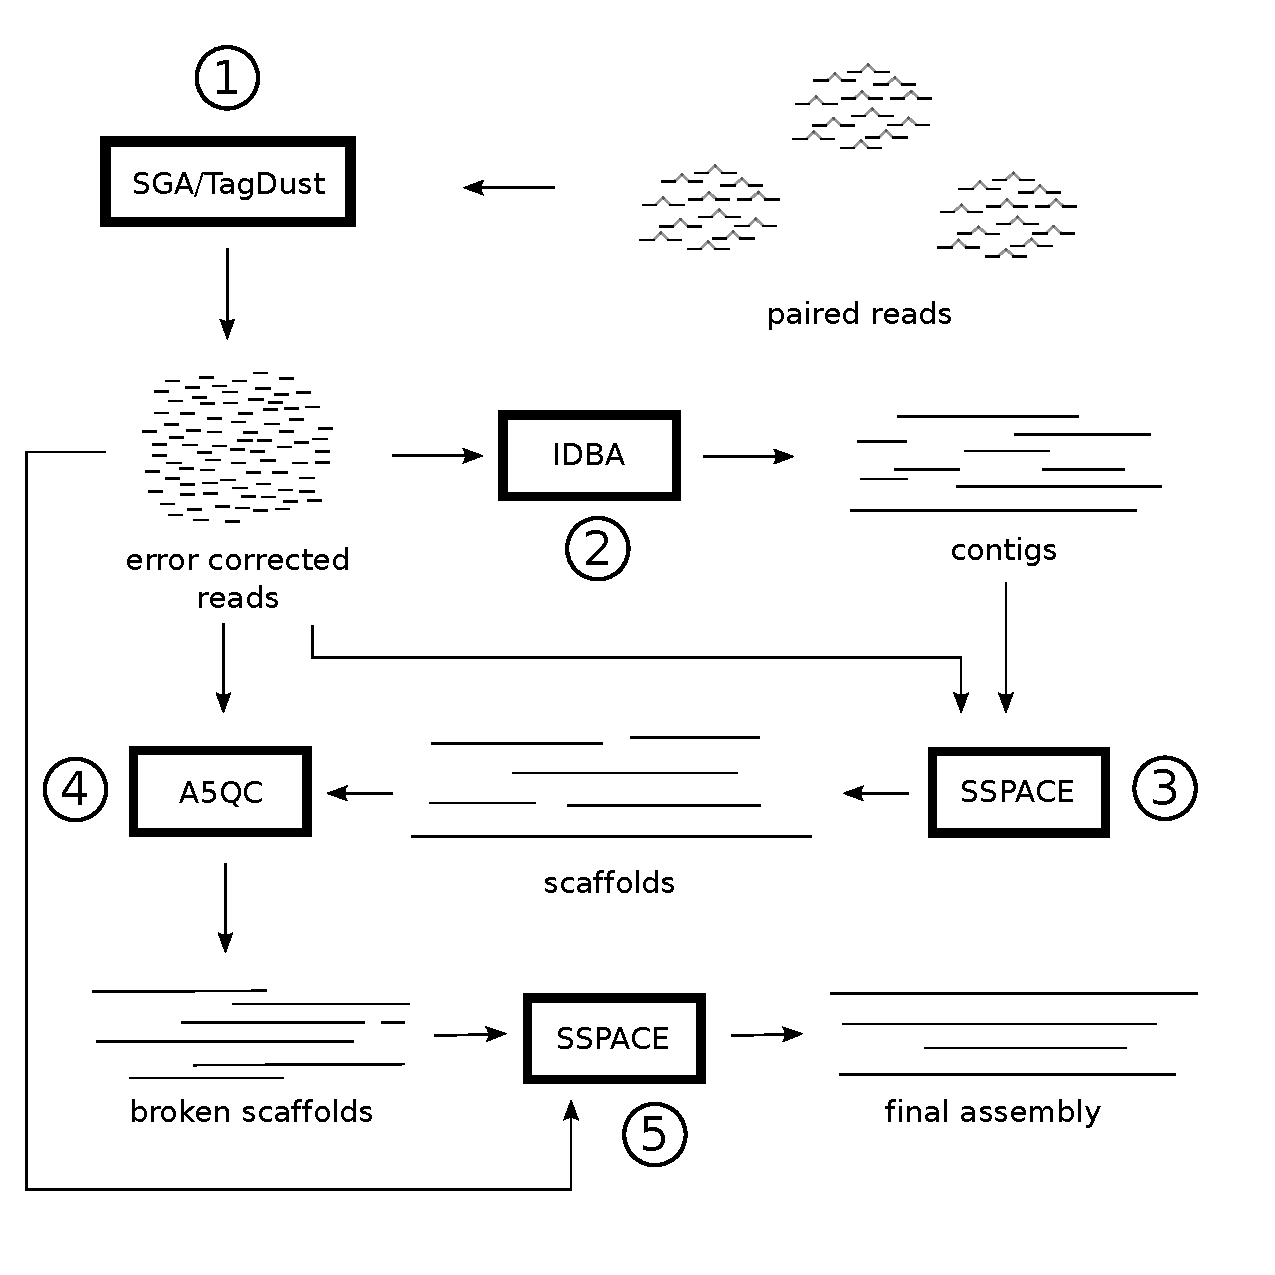
\includegraphics[width=3.5in]{a5pipeline-diagram.pdf}
\vspace{-1cm}
\caption{Diagram of pipeline. }\label{fig:01}
\end{figure}

\begin{figure}[t]
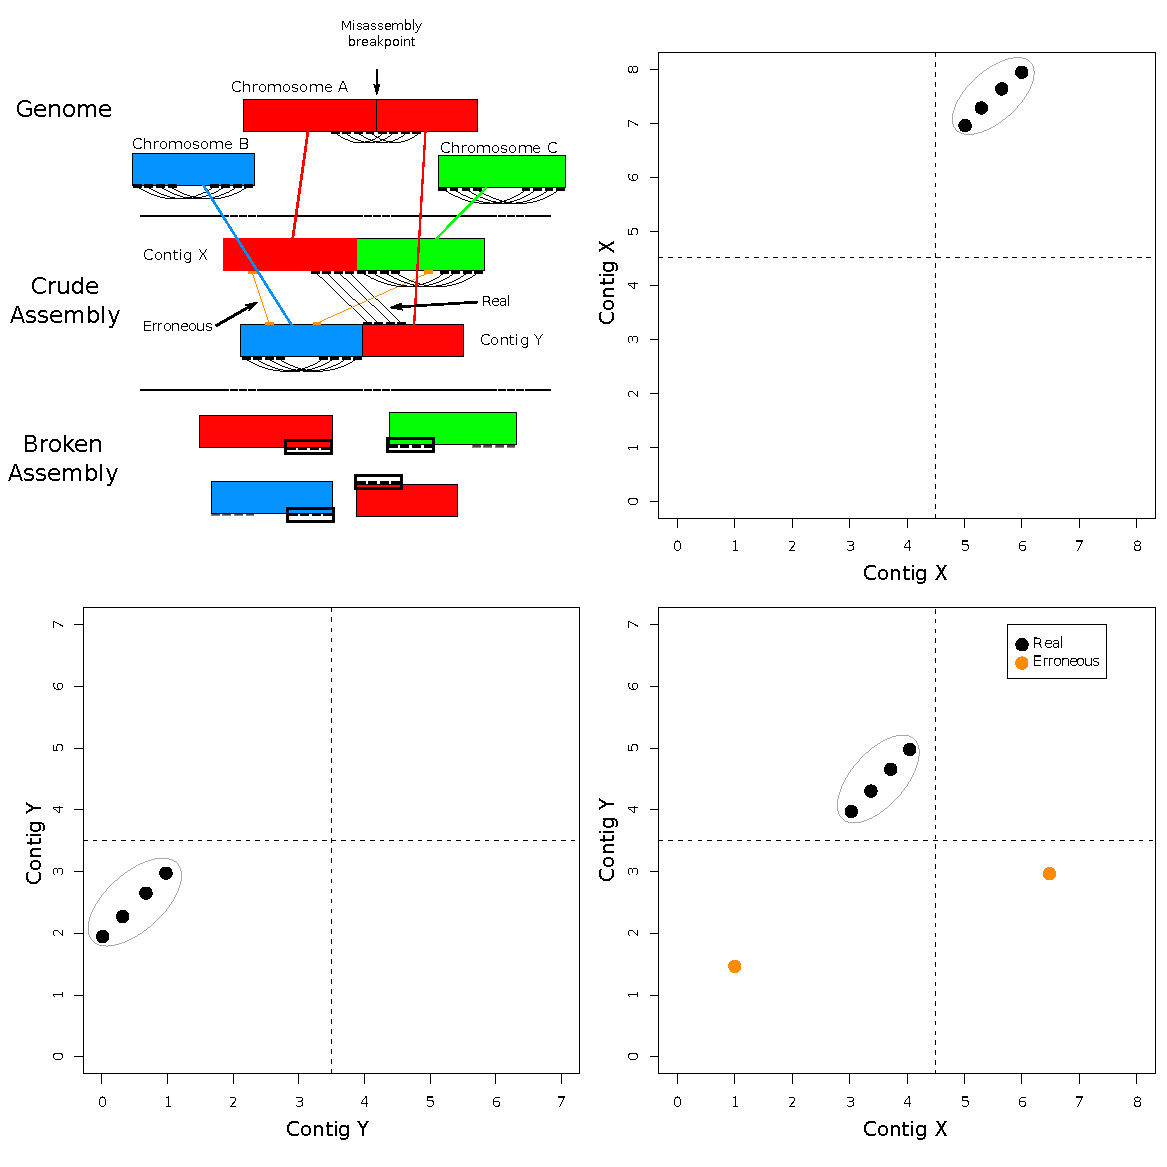
\includegraphics[width=3.5in]{fish-qc.pdf}
\vspace{-1cm}
\caption{\textbf{Left:} Topology of misassemblies in de novo genome assemblies. Orange and black lines represent paired read 
connections. \textbf{Right:} Plot of points of connections by paired reads between Contig X and Contig Y. Vertical and horizontal 
dashed lines represent locations of misassemblies in Contig X and Contig Y, repsectively. The gray circle represents the string of points
that is identified using FISH. Orange and black points correspond to orange and black lines on left.}\label{fig:02}
\end{figure}




\section*{Acknowledgements}
This work was supported by National Science Foundation award ER 0949453.

\bibliographystyle{natbib}
\bibliography{ngopt-appnote}

\end{document}
